\documentclass[border=4pt]{standalone}
\usepackage{amsmath,amssymb,amsfonts}
\usepackage{xcolor,colortbl,array,booktabs,multirow}
\usepackage{tikz}
\usepackage{pgfplots}
\pgfplotsset{compat=1.16}
\usetikzlibrary{arrows, automata, backgrounds, calendar, chains, decorations,
    matrix, mindmap, patterns, petri, positioning, shadows, shapes.geometric,
    trees, shapes, decorations.pathreplacing, calc, tikzmark, arrows.meta,
    intersections, fit, graphs, quotes, angles, decorations.markings}
\newcommand{\st}{\text{ s.t. }}
\newcommand{\x}{\mathbf{x}}
\renewcommand{\b}{\mathbf{b}}
\renewcommand{\c}{\mathbf{c}}
\newcommand{\A}{\mathbf{A}}
\newcommand{\y}{\mathbf{y}}
\newcommand{\z}{\mathbf{z}}
\newcommand{\R}{\mathbb{R}}
\newcommand{\RR}{\mathbb{R}}
\newcommand{\Z}{\mathbb{Z}}
\newcommand{\ZZ}{\mathbb{Z}}
\newcommand{\npcomplete}{NP-complete}
\providecommand{\true}{\text{TRUE}}
\providecommand{\false}{\text{FALSE}}
\tikzset{vertex/.style={circle,fill=black!25,minimum size=20pt,inner sep=0pt},
    edge/.style={draw,thick,-},weight/.style={font=\small},
    selected vertex/.style={vertex, fill=red!24},
    selected edge/.style={draw,line width=2pt,-,red!50},
    ignored edge/.style={draw,line width=2pt,-,black!20}}
\newcommand{\vect}{\vec}
\providecommand{\ds}{\displaystyle}
\providecommand{\longvect}{\overrightarrow}
\usepackage[normalem]{ulem}
\definecolor{ocre}{RGB}{243,102,25}
\providecommand{\leftB}{\left[}
\providecommand{\rightB}{\right]}
\tikzset{directed/.style={postaction={decorate,decoration={markings,mark=at position .65 with {\arrow{>}}}}},
    directed1/.style={postaction={decorate,decoration={markings,mark=at position .65 with {\arrow{>}}}}}}
\begin{document}
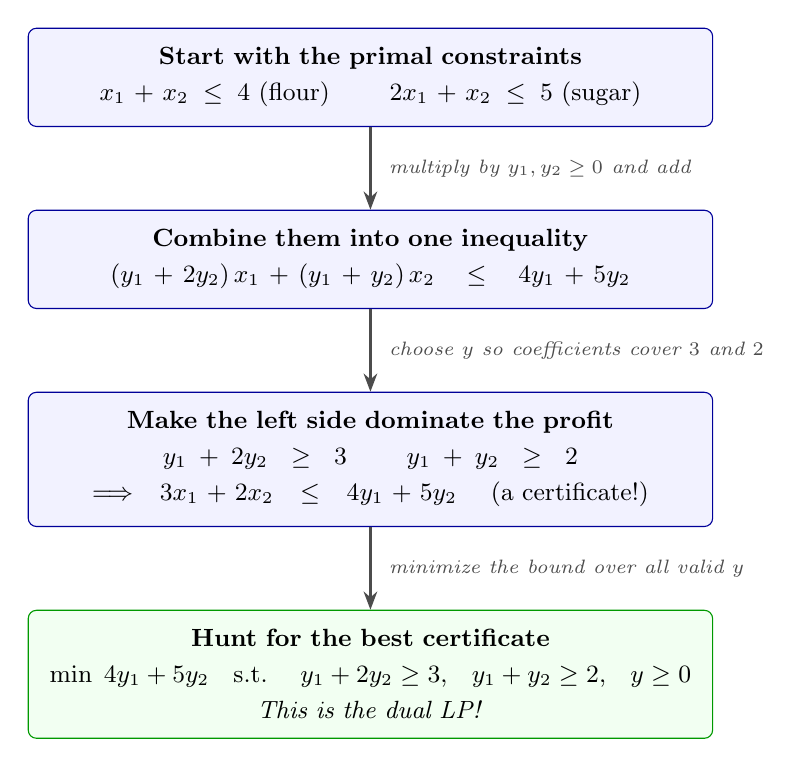
\begin{tikzpicture}[
    node distance=1.05cm,
    box/.style={rectangle, rounded corners=3pt, draw=blue!60!black, fill=blue!5,
                text width=8.2cm, align=center, inner sep=7pt, font=\small},
    dualbox/.style={rectangle, rounded corners=3pt, draw=green!60!black, fill=green!5,
                text width=8.2cm, align=center, inner sep=7pt, font=\small},
    lbl/.style={font=\scriptsize\itshape, text=black!70, align=left},
    arr/.style={-{Stealth}, thick, draw=black!70}
]
\node[box] (constraints) {\textbf{Start with the primal constraints}\\[2pt]
  $x_1 + x_2 \leq 4$ (flour) \qquad $2x_1 + x_2 \leq 5$ (sugar)};
\node[box, below=of constraints] (combine) {\textbf{Combine them into one inequality}\\[2pt]
  $(y_1 + 2y_2)\,x_1 + (y_1 + y_2)\,x_2 \;\leq\; 4y_1 + 5y_2$};
\node[box, below=of combine] (dominate) {\textbf{Make the left side dominate the profit}\\[2pt]
  $y_1 + 2y_2 \geq 3$ \qquad $y_1 + y_2 \geq 2$\\[2pt]
  $\Longrightarrow\; 3x_1 + 2x_2 \;\leq\; 4y_1 + 5y_2$ \quad (a certificate!)};
\node[dualbox, below=of dominate] (dual) {\textbf{Hunt for the best certificate}\\[2pt]
  $\min\; 4y_1 + 5y_2$ \; s.t. \; $y_1 + 2y_2 \geq 3$, \; $y_1 + y_2 \geq 2$, \; $y \geq 0$\\[2pt]
  \emph{This is the dual LP!}};
\draw[arr] (constraints) -- node[lbl, right=3pt] {multiply by $y_1, y_2 \geq 0$ and add} (combine);
\draw[arr] (combine) -- node[lbl, right=3pt] {choose $y$ so coefficients cover $3$ and $2$} (dominate);
\draw[arr] (dominate) -- node[lbl, right=3pt] {minimize the bound over all valid $y$} (dual);
\end{tikzpicture}
\end{document}
